\documentclass[11pt,reqno]{amsart}

\usepackage[a4paper,margin=28mm]{geometry}
\usepackage[T1]{fontenc}
\usepackage{lmodern}
\usepackage{microtype}
\usepackage{amsmath,amssymb,amsfonts,mathtools}
\usepackage{booktabs,array,tabularx,longtable}
\usepackage{enumitem}
\usepackage{xcolor}
\usepackage{tikz}
\usetikzlibrary{arrows.meta,positioning,calc,fit,shapes.geometric}
\usepackage{hyperref}
\usepackage[nameinlink,noabbrev]{cleveref}
\usepackage{url}
\usepackage{listings}

\definecolor{DeepBlue}{RGB}{28,63,120}
\definecolor{SoftBlue}{RGB}{236,242,251}
\definecolor{SoftGold}{RGB}{251,246,228}
\definecolor{SoftGreen}{RGB}{237,248,240}
\definecolor{SoftRed}{RGB}{252,239,239}
\hypersetup{
  colorlinks=true,
  linkcolor=DeepBlue,
  citecolor=DeepBlue,
  urlcolor=DeepBlue,
  pdfauthor={Fabian Franz and GPT-5.6 Pro},
  pdftitle={Projectors and Unit Defect in the Proposed Complex Six-Sphere Construction, Version 2}
}

\setlist[itemize]{leftmargin=2em,itemsep=0.25em,topsep=0.35em}
\setlist[enumerate]{leftmargin=2.2em,itemsep=0.3em,topsep=0.35em}
\allowdisplaybreaks
\numberwithin{equation}{section}

\newcommand{\Z}{\mathbb Z}
\newcommand{\Q}{\mathbb Q}
\newcommand{\R}{\mathbb R}
\newcommand{\C}{\mathbb C}
\newcommand{\Pone}{\mathbb P^1}
\newcommand{\Id}{\mathrm{Id}}
\newcommand{\im}{\operatorname{im}}
\newcommand{\rk}{\operatorname{rk}}
\newcommand{\coker}{\operatorname{coker}}
\newcommand{\SNF}{\operatorname{SNF}}
\newcommand{\dP}{\mathrm{dP}_6}
\newcommand{\NS}{\operatorname{NS}}
\newcommand{\Pic}{\operatorname{Pic}}
\newcommand{\Aut}{\operatorname{Aut}}
\newcommand{\vol}{\operatorname{vol}}
\newcommand{\Tor}{\operatorname{Tor}}
\newcommand{\Def}{\operatorname{Def}}
\newcommand{\eps}{\varepsilon}
\newcommand{\epsp}{\varepsilon'}
\newcommand{\wideg}{\widehat\gamma}
\newcommand{\wideu}{\widehat u}
\newcommand{\widew}{\widehat w}
\newcommand{\wided}{\widehat\delta}
\newcommand{\LambdaTor}{\Lambda_{\mathrm{tor}}}
\newcommand{\LCP}{\mathsf{LCP}}

\newtheorem{theorem}{Theorem}[section]
\newtheorem{proposition}[theorem]{Proposition}
\newtheorem{lemma}[theorem]{Lemma}
\newtheorem{corollary}[theorem]{Corollary}
\newtheorem{construction}[theorem]{Construction package}
\theoremstyle{definition}
\newtheorem{principle}[theorem]{Principle}
\newtheorem{definition}[theorem]{Definition}
\newtheorem{remark}[theorem]{Remark}
\newtheorem{question}[theorem]{Question}

\newenvironment{statusnote}{%
  \begin{center}\begin{minipage}{0.94\textwidth}\small\hrule\vspace{0.7em}%
}{%
  \vspace{0.7em}\hrule\end{minipage}\end{center}%
}

\newenvironment{proofbox}{%
  \begin{center}\begin{minipage}{0.94\textwidth}\setlength{\parindent}{0pt}\small%
}{%
  \end{minipage}\end{center}%
}

\title[Projectors and unit defect for the proposed complex $S^6$]{Projectors and Unit Defect in the Proposed Complex Six-Sphere Construction\\[4pt]
\large A short proof, a historical account, and reusable formal interfaces}

\author{Fabian Franz}
\author{GPT-5.6 Pro}
\thanks{This note was produced in a human--AI collaboration. Fabian Franz supplied the structural reading and directed the mathematical compression. GPT-5.6 Pro developed the shortcut lemmas, checked the finite calculations, and prepared the manuscript and formalization scaffold. Publication and mathematical responsibility remain with the human author and any subsequent reviewers.}
\date{27 August 2026 \;---\; version 2}

\subjclass[2020]{32J17, 14D06, 14M25, 55T10, 57R55}
\keywords{six-sphere, complex structure, torus fibration, triangle group, logarithmic transform, toric degeneration, Reynolds projector, Leray spectral sequence, formal verification}

\begin{document}

\begin{abstract}
A recent 108-page manuscript proposes a compact complex threefold $X$ diffeomorphic to the standard six-sphere. Its construction is explicit but difficult to audit as a single argument. We give a short structural proof of its global recognition theorem, conditional on an explicitly isolated local analytic construction package, and place the construction in its useful mathematical lineage: logarithmic transforms of elliptic fibrations, toric degenerations of tori, Seifert-type multiplicity arithmetic, and high-dimensional sphere recognition.

The main simplification is that the two translation twists are not ad hoc fixed vectors. They are the normalized cyclic averages of one primitive lattice vector:
\[
 v_1=P_3\wideg,\qquad v_2=-P_4\wideg,
 \qquad
 P_m=\frac1m\sum_{k=0}^{m-1}A^k.
\]
The cusp is controlled by a square-zero exchange operator and a unimodular map $B_0$; the global topology is controlled by a second unimodular certificate,
\[
 p=12\ell_0-4\ell_1-3\ell_2=-1.
\]
The first unit makes the toric central fibre irreducible and gives Euler number $2$. The second unit kills the fundamental group and all middle integral cohomology.

The argument is presented twice. Section~4 gives the concise mathematical proof and names its non-simplifiable analytic residue. Section~5 gives the same conditional recognition in a historical and human-readable register. Section~6 exports generic averaging, exchange, gluing, transgression, component-count, and conductor results, states formalization interfaces, and records lessons for reuse. A Lean formalization of the finite matrix and arithmetic core is underway; this version makes no machine-verification claim until that development has compiled and been reviewed without gaps.
\end{abstract}

\maketitle
\tableofcontents

\begin{statusnote}
\textbf{Verification status.}
The source manuscript~\cite{S6} is not yet independently certified and its conclusion conflicts with a published result of Campana--Demailly--Peternell~\cite{CDP20}. This paper is therefore not presented as an independent community verification of the existence of a complex structure on $S^6$. It does three narrower things: it states the exact local analytic package on which the construction rests; it gives a new, short derivation of the twists and of the global topological recognition; and it extracts reusable mathematical interfaces from the finite algebraic core. A Lean formalization is in progress, but is not counted as verified in this version. If the local package is independently verified, the proof below closes the theorem.
\end{statusnote}

\section{The problem revisited}\label{sec:problem}

\subsection{From an integrability problem to a recognition problem}

Hopf's question asks whether the smooth six-sphere admits an integrable complex structure~\cite{Hopf}. The familiar octonionic almost-complex structure does not solve this problem: it is not integrable. A direct attack would therefore begin with a tensor $J$ on the already known sphere and attempt to prove that its Nijenhuis tensor vanishes.

The proposed construction reverses the direction. It first builds a compact complex threefold $X$ by holomorphic gluing and only afterwards asks which smooth six-manifold underlies it:
\[
\text{holomorphic local models}
\longrightarrow
\text{compact complex threefold }X
\longrightarrow
\text{smooth recognition}.
\]
Integrability is automatic in the first arrow because all charts and transition maps are holomorphic. The difficult global question becomes topological: prove that $X$ is the standard $S^6$.

This reversal is the first conceptual economy of the proof. It changes the main unknown from a nonlinear differential equation on $S^6$ to a gluing and recognition problem for a complex fibration.

\subsection{What now exists}

A concrete proof proposal now exists~\cite{S6}; a separate AI-assisted distillation gives a useful audit map of its architecture~\cite{Feng}. It constructs a fibration
\[
 f:X\longrightarrow \Pone
\]
whose generic fibres are complex two-tori. There are exactly three exceptional fibres, corresponding to the three special points of the triangle orbifold $\Pone(3,4,\infty)$:
\begin{itemize}
\item a multiple bielliptic fibre $3S_1$ at the order-three point;
\item a multiple bielliptic fibre $4S_2$ at the order-four point;
\item a reduced non-normal toric fibre $W$ at the cusp.
\end{itemize}
The normalization of $W$ is the degree-six del Pezzo surface, with opposite sides of its anticanonical hexagon identified. Its two triple points carry the entire Euler characteristic:
\[
 e(X)=e(W)=2.
\]
The source then computes $\pi_1(X)$ and the integral homology, and recognizes $X$ as the standard six-sphere.

The challenge has consequently changed. It is no longer only to invent a possible geometry; it is to expose the load-bearing claims, shorten the finite calculations, and formalize enough of the argument that errors cannot hide in conventions.

\subsection{The precise theorem proved in this note}

We separate local complex geometry from global recognition. The following package is the precise import from the local and integral parts of the source manuscript~\cite[\S\S2--7]{S6}.

\begin{construction}[Local analytic construction package $\LCP$]\label{pkg:lcp}
Let $V\cong\Z^4$ have basis $(\gamma,u,w,\delta)$, let $\Lambda=V^*$ have dual basis $(\wideg,\wideu,\widew,\wided)$, and let $T_1,T_2$ be the matrices in \cref{sec:lattice}. Put $A_j=(T_j^{-1})^t$ and $T_0=(T_1T_2)^{-1}=I+N$.

The package $\LCP$ consists of the following assertions.
\begin{enumerate}[label=\textup{(L\arabic*)}]
\item \textbf{Open period family.} There are holomorphic functions $\tau,\mu,\beta$ on the upper half-plane satisfying the prescribed triangle-group transformation laws such that
\[
 \Pi(z)=
 \begin{pmatrix}
 6\mu(z)&\tau(z)&1&0\\
 \beta(z)&\mu(z)&0&1
 \end{pmatrix}
\]
defines a proper holomorphic family $J\to B^\circ$ of complex two-tori over
$B^\circ=\Pone\setminus\{p_0,p_1,p_2\}$, with monodromies $A_1,A_2,M_0$.

\item \textbf{Cusp normal form and toric filling.} Near $p_0$ the period matrix has the form
\[
 [\,sB_0+C(t_c)\mid I\,],
\]
where $C$ extends holomorphically to $t_c=0$ and
\[
 B_0:\Lambda/\LambdaTor\xrightarrow{\sim}\LambdaTor,
 \qquad
 \LambdaTor=\langle\widew,\wided\rangle,
\]
is the unimodular map
\[
 B_0(\overline{\wideg})=-\wided,
 \qquad
 B_0(\overline{\wideu})=\widew.
\]
The associated $A_2$-toric quotient is a smooth complex threefold over a disc, agrees with $J$ over the punctured disc, and has reduced irreducible central fibre $W$ whose normalization is $\dP$, with three double curves and two triple points.

\item \textbf{Finite-monodromy fillings.} For the invariant primitive vectors
\[
 v_1=\wideg+2\wideu-4\widew,
 \qquad
 v_2=-(\wideg+3\wideu-3\widew),
\]
the order-three and order-four logarithmic transforms are free. They produce smooth local threefolds with multiple fibres $3S_1$ and $4S_2$, and agree with $J$ over the punctured discs.

\item \textbf{Integral specialization.} The specialization maps at the cusp and the two finite-monodromy points identify the integral lattices in $R^qf_*\Z$ stated in \cref{sec:cohomology}. In particular, the only relevant Leray differentials are the three rank-one maps computed from the same gluing integer $p$.
\end{enumerate}
\end{construction}

The source manuscript proves a much larger theorem. The package above is deliberately smaller: it contains exactly the analytic and local-topological information that the short global proof needs.

\begin{theorem}[Short recognition theorem]\label{thm:main}
Every compact complex threefold obtained from $\LCP$ with the tautological cusp gluing and the projected twists $v_1,v_2$ is diffeomorphic to the standard six-sphere.
\end{theorem}

\begin{proof}
The proof occupies \cref{sec:proof}. Its finite core is the following chain.
The cusp exchange is square-zero and $B_0$ is unimodular. The finite twists are cyclic averages of the single seed $\wideg$, hence their surviving coinvariant values are $1$ and $-1$. The gluing defect is therefore
\[
 p=12\cdot0-4\cdot1-3(-1)=-1.
\]
The corresponding van Kampen relations trivialize $\pi_1(X)$. The integral Leray transgressions are multiplication by the same unit $p$, so every middle cohomology group vanishes. The toric fibre has Euler characteristic $2$. Thus $X$ is a simply connected integral homology six-sphere, hence a homotopy six-sphere; high-dimensional Poincar\'e recognition and $\Theta_6=0$ identify it diffeomorphically with the standard $S^6$.
\end{proof}

\begin{corollary}[Conditional resolution of the Hopf problem]\label{cor:conditional}
If the local analytic construction package $\LCP$ is correct, then the standard smooth six-sphere admits an integrable complex structure.
\end{corollary}

\section{Structure and declared dependencies}\label{sec:dependencies}

A short proof is useful only if it does not conceal its dependencies. This section records the mathematical ``software stack''.

\subsection{Dependency table}

\begin{center}
\small
\begin{tabularx}{\textwidth}{@{}>{\raggedright\arraybackslash\bfseries}p{0.22\textwidth}X>{\raggedright\arraybackslash}p{0.19\textwidth}@{}}
\toprule
Package & What it supplies & Status in this note\\
\midrule
Triangle orbifolds & The base $\Pone(3,4,\infty)$ and generators of orders $3,4$ with parabolic product & Standard background\\
Integer linear algebra & Monodromy matrices, fixed lattices, coinvariants, determinants, Smith normal form & Reproved; finite certificates formalized\\
Cohomology on $\Pone$ & Existence and uniqueness of the correction terms $\mu,\beta$ as torsor sections & Part of $\LCP$; proof architecture explained\\
Complex tori and periods & The open family $J\to B^\circ$ from $\Pi(z)\Z^4\subset\C^2$ & Part of $\LCP$\\
Toric geometry & The $A_2$ fan, the quotient degeneration, and the self-glued $\dP$ fibre $W$ & Part of $\LCP$; component count shortened\\
Logarithmic transforms & The multiple fibres $3S_1,4S_2$ and their translation twists & Part of $\LCP$; twist selection shortened\\
Van Kampen and Smith theory & The fundamental group and the defect integer $p$ & Reproved in full\\
Nearby cycles and integral Leray & The specialization lattices and the three transgressions & Local data in $\LCP$; abstract unit argument reproved\\
High-dimensional topology & Homology sphere $\Rightarrow$ standard smooth $S^6$ & Standard theorems\\
\bottomrule
\end{tabularx}
\end{center}

\subsection{Architecture}

\begin{figure}[ht]
\centering
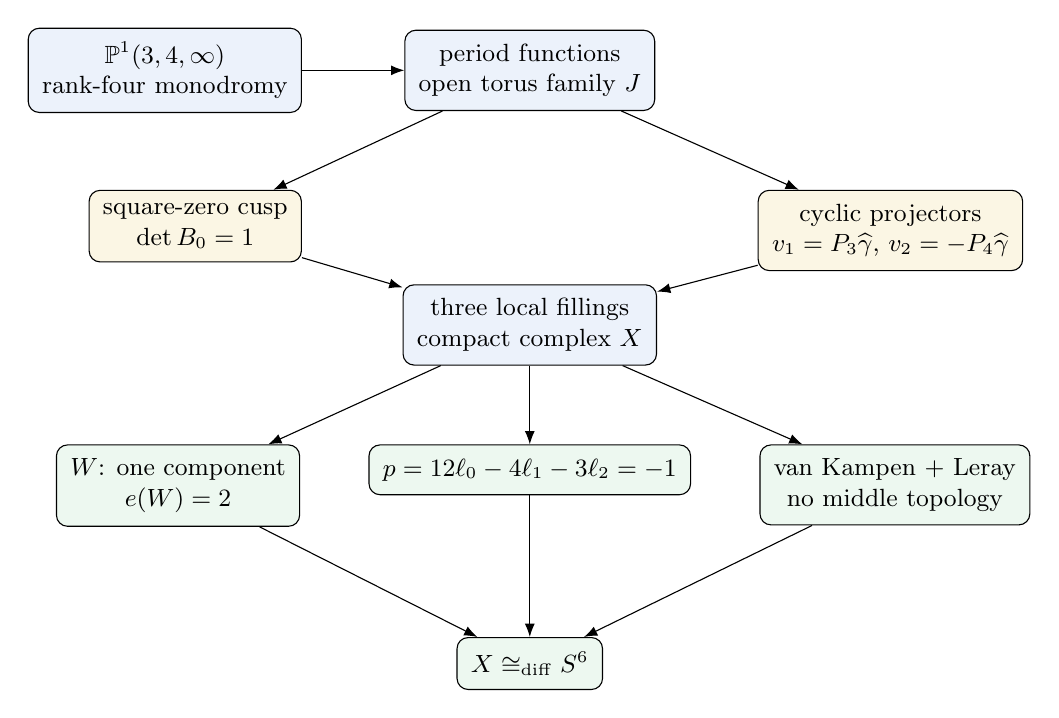
\begin{tikzpicture}[
  >=Latex,
  node distance=10mm and 13mm,
  box/.style={draw,rounded corners,align=center,inner sep=5pt,font=\small},
  local/.style={box,fill=SoftBlue},
  finite/.style={box,fill=SoftGold},
  global/.style={box,fill=SoftGreen}
]
\node[local] (orb) {$\Pone(3,4,\infty)$\\rank-four monodromy};
\node[local,right=of orb] (period) {period functions\\open torus family $J$};
\node[finite,below left=of period] (cusp) {square-zero cusp\\$\det B_0=1$};
\node[finite,below right=of period] (proj) {cyclic projectors\\$v_1=P_3\wideg$, $v_2=-P_4\wideg$};
\node[local,below=22mm of period] (fill) {three local fillings\\compact complex $X$};
\node[global,below left=of fill] (euler) {$W$: one component\\$e(W)=2$};
\node[global,below=of fill] (defect) {$p=12\ell_0-4\ell_1-3\ell_2=-1$};
\node[global,below right=of fill] (leray) {van Kampen + Leray\\no middle topology};
\node[global,below=18mm of defect] (sphere) {$X\cong_{\mathrm{diff}}S^6$};
\draw[->] (orb)--(period);
\draw[->] (period)--(cusp);
\draw[->] (period)--(proj);
\draw[->] (cusp)--(fill);
\draw[->] (proj)--(fill);
\draw[->] (fill)--(euler);
\draw[->] (fill)--(defect);
\draw[->] (fill)--(leray);
\draw[->] (euler)--(sphere);
\draw[->] (defect)--(sphere);
\draw[->] (leray)--(sphere);
\end{tikzpicture}
\caption{The compressed architecture. Blue nodes are the local analytic construction package; gold nodes are the new finite shortcuts; green nodes are the global recognition.}
\label{fig:architecture}
\end{figure}

\subsection{What is and is not shortened}

The shortcuts do not make properness, freeness, holomorphic extension, or integral specialization disappear. Those are genuine geometric statements. They do remove three kinds of avoidable complexity:
\begin{enumerate}
\item fixed vectors at the finite points are produced canonically by averaging rather than guessed and solved for;
\item the cusp matrices are recognized as a universal square-zero two-channel exchange rather than repeatedly expanded;
\item the global topology is organized by two integers, $d=|\det B_0|$ and $p=12\ell_0-4\ell_1-3\ell_2$, instead of by a long list of attaching calculations.
\end{enumerate}

\section{Focus: the proof in one page}\label{sec:focus}

\begin{proofbox}
\textbf{Step 1: Create the open complex world.}
Use the triangle group $\Delta(3,4,\infty)$ and the period matrix $\Pi(z)$ to build a holomorphic family of complex two-tori over the thrice-punctured sphere.

\medskip
\textbf{Step 2: Identify the obstruction.}
The monodromy preserves an alternating form, but the associated symmetric form at the cusp has signature $(1,1)$. Hence the family is not polarizable, so the usual positive compactification theorems do not apply. An explicit cusp world is required.

\medskip
\textbf{Step 3: Linearize the cusp.}
The cusp monodromy is $I+N$ with $N^2=0$. Thus the exchange flow is exactly $I+sN$, with no higher terms. On the dual lattice it transfers one rank-two quotient isomorphically onto one rank-two toric lattice. The transfer matrix $B_0$ has determinant $1$.

\medskip
\textbf{Step 4: Project to the finite fixed lattices.}
For a finite-order monodromy $A$, the uniform orbit average
\[
P_m=\frac1m(I+A+\cdots+A^{m-1})
\]
is the projector onto the fixed subspace. Applied to the same primitive seed $\wideg$, it gives exactly the two integral twist vectors required by the logarithmic transforms.

\medskip
\textbf{Step 5: Close the three punctures.}
Use the $A_2$ toric quotient at the cusp and the order-three and order-four logarithmic transforms at the finite points. Holomorphic gluing produces a compact complex threefold $X$.

\medskip
\textbf{Step 6: Read the singular sample.}
The quotient triangulation has one vertex orbit, three edge orbits, and two triangle orbits. Thus the central fibre has one component, three double curves, and two triple points, and
\[
e(W)=e((\C^*)^2)+3e(\C^*)+2=2.
\]

\medskip
\textbf{Step 7: Solve the arithmetic.}
The invariant functional $\gamma$ survives orbit averaging. Therefore
\[
(\ell_0,\ell_1,\ell_2)=(0,1,-1),
\qquad p=12\ell_0-4\ell_1-3\ell_2=-1.
\]
The van Kampen relations collapse in three lines, and $\pi_1(X)=1$.

\medskip
\textbf{Step 8: Use the same unit in cohomology.}
The three integral Leray transgressions are multiplication by $p$. Since $p=-1$, they are isomorphisms. All middle integral cohomology vanishes.

\medskip
\textbf{Step 9: Recognize the result.}
The compact smooth six-manifold $X$ is simply connected and has the homology of $S^6$. It is a homotopy sphere, and $\Theta_6=0$ implies that it is diffeomorphic to the standard sphere.
\end{proofbox}

The rest of the paper justifies each compression and explains why the same small set of certificates appears in several mathematical languages.

\section{Presentation of the short proof}\label{sec:proof}

\subsection{The rank-four lattice and the non-polarizable obstruction}\label{sec:lattice}

In the basis $(\gamma,u,w,\delta)$ of $V\cong\Z^4$, take
\begin{equation}\label{eq:T1T2}
T_1=
\begin{pmatrix}
1&0&-6&2\\
0&-1&1&1\\
0&-1&0&1\\
0&0&0&1
\end{pmatrix},
\qquad
T_2=
\begin{pmatrix}
1&6&0&-3\\
0&0&-1&1\\
0&1&0&0\\
0&0&0&1
\end{pmatrix}.
\end{equation}
Direct multiplication gives
\[
 T_1^3=I,
 \qquad
 T_2^4=I,
\]
and
\begin{equation}\label{eq:N}
T_0=(T_1T_2)^{-1}=I+N,
\qquad
N=
\begin{pmatrix}
0&0&0&1\\
0&0&-1&0\\
0&0&0&0\\
0&0&0&0
\end{pmatrix},
\qquad N^2=0.
\end{equation}
Thus $N\delta=\gamma$, $Nw=-u$, and $N\gamma=Nu=0$.

The primitive invariant alternating form is represented by
\begin{equation}\label{eq:Q0}
Q_0=
\begin{pmatrix}
0&0&0&1\\
0&0&6&0\\
0&-6&0&0\\
-1&0&0&0
\end{pmatrix}.
\end{equation}
One checks
\[
T_j^tQ_0T_j=Q_0
\quad(j=1,2),
\qquad
N^tQ_0+Q_0N=0.
\]
By \cref{lem:square-zero-exchange}, the exact exchange flow
\[
E_s=I+sN
\]
preserves $Q_0$ for every scalar $s$.

On $V/\ker N$, the symmetric form
\[
 b_N(x,y)=Q_0(x,Ny)
\]
has Gram matrix $\operatorname{diag}(6,-1)$ in a suitable basis. It has signature $(1,1)$. This is the hard analytic obstruction: the construction conserves an alternating pairing, but not a positive polarization. Standard polarized degeneration theory cannot be invoked as a black box. The explicit toric filling in $\LCP$ is therefore essential rather than decorative.

\subsection{The cusp is a complete rank-two exchange}

Pass to the dual lattice $\Lambda=V^*$. The finite monodromies are
\begin{equation}\label{eq:A1A2}
A_1=(T_1^{-1})^t=
\begin{pmatrix}
1&0&0&0\\
6&0&1&0\\
-6&-1&-1&0\\
-2&1&0&1
\end{pmatrix},
\qquad
A_2=(T_2^{-1})^t=
\begin{pmatrix}
1&0&0&0\\
0&0&-1&0\\
-6&1&0&0\\
3&0&1&1
\end{pmatrix}.
\end{equation}
At the cusp, $M_0=(T_0^{-1})^t=I-N^t$. Put
\[
D=M_0-I=-N^t.
\]
Then
\[
D^2=0,
\qquad
\ker D=\im D=\LambdaTor=\langle\widew,\wided\rangle.
\]
The induced map
\[
B_0:\Lambda/\LambdaTor\longrightarrow\LambdaTor
\]
sends
\[
\overline{\wideg}\longmapsto-\wided,
\qquad
\overline{\wideu}\longmapsto\widew.
\]
In the displayed bases,
\begin{equation}\label{eq:B0}
[B_0]=
\begin{pmatrix}
0&1\\
-1&0
\end{pmatrix},
\qquad
\det B_0=1.
\end{equation}
Equivalently, $D$ has Smith normal form $\operatorname{diag}(1,1,0,0)$. After an integral change of basis the cusp module is simply two copies of the dual-number module $\Z[\epsilon]/(\epsilon^2)$.

This observation shortens the cusp algebra. There is no hidden higher-order nilpotent structure: two independent directions transfer once, integrally and completely, into two vanishing directions.

\subsection{The twist vectors are canonical orbit averages}\label{sec:projectors}

For a finite-order operator $A$ of order $m$, define its cyclic averaging operator
\[
P_m(A)=\frac1m\sum_{k=0}^{m-1}A^k.
\]
By \cref{lem:cyclic-projector}, this is an idempotent projector onto the fixed subspace over $\Q$.

For the two matrices in \cref{eq:A1A2}, direct calculation gives
\begin{equation}\label{eq:P3P4}
P_3=
\begin{pmatrix}
1&0&0&0\\
2&0&0&0\\
-4&0&0&0\\
0&\frac23&\frac13&1
\end{pmatrix},
\qquad
P_4=
\begin{pmatrix}
1&0&0&0\\
3&0&0&0\\
-3&0&0&0\\
0&\frac12&\frac12&1
\end{pmatrix}.
\end{equation}
They are rational projectors, but their values on the primitive seed $\wideg$ are integral:
\begin{equation}\label{eq:projected-twists}
P_3\wideg=\wideg+2\wideu-4\widew=:\eps,
\qquad
P_4\wideg=\wideg+3\wideu-3\widew=:\epsp.
\end{equation}
Moreover,
\[
A_1\eps=\eps,
\qquad
A_2\epsp=\epsp.
\]
Thus the twists required by the logarithmic transforms can be chosen canonically as
\begin{equation}\label{eq:v1v2}
v_1=P_3\wideg=\eps,
\qquad
v_2=-P_4\wideg=-\epsp.
\end{equation}

The surviving coinvariant functional is evaluation against $\gamma\in V$:
\[
\gamma:\Lambda\longrightarrow\Z,
\qquad
\gamma(a\wideg+b\wideu+c\widew+d\wided)=a.
\]
It is invariant under both monodromies. Hence \cref{lem:observable} gives
\begin{equation}\label{eq:ell-values}
\ell_1:=\gamma(v_1)=1,
\qquad
\ell_2:=\gamma(v_2)=-1.
\end{equation}
The tautological cusp gluing has $\ell_0=0$.

This is the main new algebraic shortcut. The fixed vectors, their primitivity, and their global signs are all generated from one seed by a universal operation: finite-orbit averaging.

\subsection{Closing the three punctures}

The open family $J\to B^\circ$ is completed according to monodromy type.

At the cusp, the $A_2$-triangulation of $\R^2$ defines an infinite smooth toric threefold. The regular term $C(t_c)$ in the cusp period normal form corrects the lattice action, and $B_0$ identifies the acting lattice with the translation lattice. Since $B_0$ is unimodular, \cref{lem:component-index} implies that there is one vertex orbit and hence one irreducible component downstairs.

At the two finite points, the order-three and order-four deck rotations are coupled with $A_1,A_2$ and translations by $v_1/3,v_2/4$. The local freeness congruences hold because $\gamma(v_1)=1$ is nonzero modulo $3$ and $\gamma(v_2)=-1$ is odd. The quotients are smooth and their central divisors are multiple fibres with smooth bielliptic reductions.

The three local models agree holomorphically with $J$ over punctured discs, so they glue to a compact connected complex threefold
\[
X=J\cup N_0\cup N_1\cup N_2
\]
with a holomorphic map $f:X\to\Pone$.

This is where the local construction package is used. From this point onwards the proof is global and short.

\subsection{The toric fibre carries exactly two units of Euler characteristic}

Modulo the lattice, the $A_2$-triangulation has
\[
1\text{ vertex orbit},
\qquad
3\text{ edge orbits},
\qquad
2\text{ triangle orbits}.
\]
The corresponding strata of the central fibre are
\[
W=(\C^*)^2\sqcup 3\C^*\sqcup 2\{\mathrm{point}\}.
\]
By additivity,
\begin{equation}\label{eq:eW}
e(W)=e((\C^*)^2)+3e(\C^*)+2=0+0+2=2.
\end{equation}
Every smooth torus fibre has Euler characteristic zero. The reduced supports of the two multiple fibres are bielliptic surfaces and also have Euler characteristic zero. By \cref{lem:euler-localization},
\begin{equation}\label{eq:eX}
e(X)=e(W)=2.
\end{equation}

Unimodularity is visible here as component control. If the image of $B_0$ had index $d>1$, there would be $d$ vertex orbits, hence $d$ components and Euler number $2d$. The equality $\det B_0=1$ is therefore the local unit certificate selecting the sphere's Euler number.

\subsection{The fundamental group collapses in three lines}\label{sec:pi1}

After the vanishing cycles and monodromy kill three fibre directions, only the coinvariant circle $c$ survives. Let $x,y$ be meridians of the order-three and order-four fibres. Van Kampen gives
\begin{equation}\label{eq:presentation}
\pi_1(X)=
\left\langle c,x,y\ \middle|\
 c\text{ central},\quad
 xy=c^{\ell_0},\quad
 x^3=c^{\ell_1},\quad
 y^4=c^{\ell_2}
\right\rangle.
\end{equation}
For the projected twists, $(\ell_0,\ell_1,\ell_2)=(0,1,-1)$. Therefore
\[
xy=1,
\qquad x^3=c,
\qquad y^4=c^{-1}.
\]
The first relation gives $y=x^{-1}$. The third then gives $x^{-4}=c^{-1}$, or $x^4=c$. Comparing with $x^3=c$ yields $x=1$. Consequently $c=y=1$.

Thus
\begin{equation}\label{eq:pi1trivial}
\pi_1(X)=1.
\end{equation}

For comparison, the generic computation of \cref{thm:gluing-group} gives
\[
\pi_1(X)\cong\Z/|p|,
\qquad
p=12\ell_0-4\ell_1-3\ell_2.
\]
The actual value is
\begin{equation}\label{eq:pminusone}
p=12\cdot0-4\cdot1-3(-1)=-1.
\end{equation}
The three-line proof above is the specialization of the Smith-normal-form calculation to a unimodular relation matrix.

\subsection{The same unit kills the middle cohomology}\label{sec:cohomology}

Consider the integral Leray spectral sequence
\[
E_2^{a,b}=H^a(\Pone,R^bf_*\Z)\Longrightarrow H^{a+b}(X;\Z).
\]
The specialization data in $\LCP$ give the relevant global generators
\[
H^0(R^1)=12\Z\gamma,
\quad
H^0(R^2)=\Z\cdot2q,
\quad
H^0(R^3)=\Z\cdot2\gamma uw,
\]
and the corresponding rank-one groups in column $a=2$. The column-$1$ terms needed in total degrees two and three vanish. Since the base is a curve, only the differentials
\[
d_2^{0,b}:E_2^{0,b}\longrightarrow E_2^{2,b-1}
\]
can be nonzero.

The first differential is a clutching obstruction. The smallest fibrewise class compatible with the order-three and order-four stabilizers is $12\gamma$. Its three boundary discrepancies are
\[
12\ell_0,
\qquad
-4\ell_1,
\qquad
-3\ell_2.
\]
Their sum is $p$, so
\begin{equation}\label{eq:first-d2}
d_2^{0,1}(12\gamma)=\pm p\,\omega,
\end{equation}
where $\omega$ generates $H^2(\Pone;\Z)$.

Multiplicativity and the integral normalization of the specialization lattices give, with one common sign,
\begin{equation}\label{eq:three-d2}
\begin{aligned}
d_2^{0,1}(12\gamma)&=\pm p\,\omega,\\
d_2^{0,2}(2q)&=\pm p\,\omega\overline\delta,\\
d_2^{0,3}(2\gamma uw)&=\pm p\,\omega[\gamma\delta].
\end{aligned}
\end{equation}
This is the only place where the integral nearby-cycle and specialization calculations of $\LCP$ enter the global proof.

Now $p=-1$. Hence every map in \cref{eq:three-d2} is an isomorphism of infinite cyclic groups. The abstract unit-transgression lemma, \cref{lem:unit-transgression}, gives
\begin{equation}\label{eq:lowcohomology}
H^1(X;\Z)=H^2(X;\Z)=H^3(X;\Z)=0.
\end{equation}
The universal coefficient theorem and Poincar\'e duality give the remaining middle groups:
\begin{equation}\label{eq:homology-sphere}
H_k(X;\Z)=
\begin{cases}
\Z,&k=0,6,\\
0,&1\leq k\leq5.
\end{cases}
\end{equation}
Thus $X$ is an integral homology six-sphere.

The key economy is conceptual: van Kampen and Leray do not produce unrelated obstructions. They compute the same gluing integer $p$ in two languages. Unit defect means both that the last loop dies and that the last cohomology classes transgress isomorphically.

\subsection{Recognition of the standard sphere}

By \cref{eq:pi1trivial,eq:homology-sphere}, $X$ is simply connected and has the integral homology of $S^6$. Hurewicz and the homology Whitehead theorem imply that $X$ is a homotopy six-sphere. Smale's high-dimensional Poincar\'e theorem identifies it topologically with $S^6$~\cite{Smale}. Finally, the group of oriented smooth homotopy six-spheres is trivial:
\[
\Theta_6=0.
\]
Therefore $X$ is diffeomorphic to the standard smooth six-sphere~\cite{KM}. Transporting the already constructed complex atlas along this diffeomorphism gives an integrable complex structure on standard $S^6$, conditional on $\LCP$.

This completes the proof of \cref{thm:main}.

\subsection{The non-simplifiable residue}\label{sec:residue}

The shortening above does not replace the local analytic construction by linear algebra. It isolates the exact obligations that still have to be checked independently:
\begin{enumerate}[label=\textup{(R\arabic*)}]
\item the period functions produce a lattice in $\C^2$ at every point and descend with the stated monodromy;
\item the regular cusp term extends holomorphically and the corrected $\Z^2$-action on the toric model is free, properly discontinuous, and gives the asserted central fibre;
\item the order-three and order-four logarithmic transforms are free and use the stated signs, primitive twists, and multiplicities;
\item the nearby-cycle stalks, specialization indices, and normalized integral generators give the three Leray transgressions of \cref{eq:three-d2} with one common sign.
\end{enumerate}
These are the non-simplifiable residue of the proof. Every shortcut in this paper begins only after these four imports have been supplied. In particular, no determinant computation can substitute for properness, holomorphic extension, or integral specialization.

\section{The construction in context: a second proof for human understanding}\label{sec:explanation}

This section gives the same conditional recognition a second time, now in the order in which one would explain it at a blackboard. The local construction package remains an explicit assumption, but every global step is made visible through a picture, a finite count, or a two-line integral calculation.

\subsection{The historical route to this design}\label{sec:history-story}

Hopf posed the complex-six-sphere problem in the 1940s~\cite{Hopf}. Borel and Serre later showed that, among spheres, only $S^2$ and $S^6$ admit almost-complex structures~\cite{BorelSerre}. The exceptional case is not accidental: octonionic multiplication gives $S^6$ a canonical and highly symmetric almost-complex structure. Yet that structure is not integrable, and the problem survived. A compact history and further references are given in~\cite{Feng}.

The next decades progressively ruled out easy worlds. A complex $S^6$ cannot be K\"ahler because $H^2(S^6;\R)=0$. LeBrun ruled out integrable complex structures orthogonal to the round metric~\cite{LeBrun}. Campana--Demailly--Peternell gave a published exclusion of positive algebraic dimension under their hypotheses~\cite{CDP20}. The proposed construction does not return to the octonionic or round route. It builds a non-K\"ahler torus fibration of algebraic dimension one and claims that a non-normal fibre invalidates a specific torsion-free reduction used in that exclusion argument~\cite{S6,Feng}. This conflict is one reason the audit boundary in \cref{sec:residue} must remain explicit.

The local moves themselves belong to a classical lineage. Degenerating a torus by an infinite toric model and then quotienting by a lattice is the higher-dimensional relative of the Tate-curve picture and Mumford's construction of degenerating abelian varieties~\cite{BHPV,Mumford}. Creating the two multiple fibres is the higher-dimensional relative of logarithmic transforms in elliptic-surface theory~\cite{BHPV}. The final integer
\[
12\ell_0-4\ell_1-3\ell_2
\]
has the same shape as the homology formula for a Seifert fibration over $S^2(3,4)$~\cite{Orlik}. Finally, once the manifold is a simply connected homology six-sphere, the last recognition step is classical high-dimensional topology~\cite{Smale,KM}.

Thus the proposal is best understood not as one unprecedented mechanism, but as a precise synthesis of classical mechanisms one complex dimension higher, with non-polarizability and non-normality supplying the genuinely unusual features.

\subsection{Build the complex manifold first}

The usual formulation invites us to stare at the sphere and search for a complex operator on its tangent spaces. The construction instead assembles a complex world from pieces that are complex from birth. Holomorphic charts do not have to be made integrable later. Once the world is compact, only its smooth identity remains unknown.

This is analogous to constructing a surface from polygons and then computing its genus. One does not first guess a metric on the final surface. One builds a consistent object and then reads its topology from the gluing.

\subsection{One complex dimension above elliptic surfaces}

An elliptic surface has a complex curve as fibre and a complex curve as base. Here the fibre is a complex two-torus, so the total space has complex dimension three:
\[
1\text{ complex base dimension}+2\text{ complex fibre dimensions}=3.
\]
In real dimensions this is
\[
2+4=6.
\]
The three local operations are higher-dimensional versions of familiar elliptic-surface mechanisms:
\begin{center}
\begin{tabular}{@{}ll@{}}
\toprule
Elliptic surface & Proposed threefold\\
\midrule
elliptic curve & complex two-torus\\
Tate or nodal degeneration & $A_2$ toric degeneration\\
multiple elliptic fibre & multiple bielliptic fibre\\
cycle of rational curves & self-glued $\dP$ surface\\
Dolgachev multiplicity arithmetic & $(3,4)$ twist arithmetic\\
\bottomrule
\end{tabular}
\end{center}
The analogy guides the local models, but it stops at polarization. The rank-four monodromy preserves only an indefinite alternating geometry. That failure is not an inconvenience that can be ignored; it is exactly why the construction can live in the non-K\"ahler world required by $b_2(S^6)=0$.

\subsection{Square-zero means the exchange happens once}

At the cusp the monodromy is $I+N$ with $N^2=0$. Algebraically, this means that applying the nontrivial part twice gives zero. The exponential therefore terminates:
\[
e^{sN}=I+sN.
\]
There are no hidden quadratic, cubic, or infinite correction terms. The cusp consists of two source directions transferred into two target directions, once.

The transfer preserves the alternating pairing $Q_0$. It does not preserve a positive energy. The associated symmetric form has one positive and one negative direction, like a saddle rather than a bowl. This explains why the standard positive compactification machinery is unavailable and why an explicit toric universe must be built.

\subsection{Finite averaging is both algebra and probability}

At a point of monodromy order $m$, a vector can move around a finite orbit
\[
v,Av,A^2v,\ldots,A^{m-1}v.
\]
Its uniform average
\[
P_mv=\frac1m\sum_{k=0}^{m-1}A^kv
\]
is fixed by $A$. Applying the average twice changes nothing, so $P_m^2=P_m$.

This can be read algebraically as a Reynolds projector or probabilistically as expectation over a uniform finite orbit. In either language, all orbit-dependent motion cancels and the invariant part remains.

The striking fact in the six-sphere data is that one and the same primitive vector $\wideg$ produces both local twists. The denominators cancel on that seed:
\[
P_3\wideg\in\Lambda,
\qquad
P_4\wideg\in\Lambda.
\]
Thus the local choices are not unrelated guesses. They are two views of a common global class through the order-three and order-four invariant projectors.

\subsection{The singular fibre is an Euler reservoir}

A torus has Euler characteristic zero. Consequently the whole smooth region of the fibration is invisible to the Euler number. The multiple bielliptic fibres are also Euler-invisible. The required value $e(S^6)=2$ must therefore be stored at the cusp.

The $A_2$ triangulation supplies exactly two zero-dimensional strata after quotienting: the two triple points. Every positive-dimensional torus stratum has Euler characteristic zero. Hence the two points contribute the entire answer.

This is why the combinatorics matters. One vertex orbit says there is one component. Three edge orbits say there are three seams. Two triangle orbits say there are two triple points. Geometry, incidence, and Euler arithmetic are three descriptions of the same finite quotient.

\subsection{A unit does more than a zero}

The proof closes not because an obstruction is set equal to zero, but because the relevant maps are units over $\Z$.

For multiplication by an integer $p$,
\[
\Z\xrightarrow{\times p}\Z,
\]
there are three qualitatively different cases:
\begin{center}
\begin{tabular}{@{}cl@{}}
\toprule
$p=0$ & the source class survives freely;\\
$|p|>1$ & a torsion residue $\Z/|p|$ survives;\\
$|p|=1$ & the map is an integral isomorphism and leaves no residue.\\
\bottomrule
\end{tabular}
\end{center}
The cusp certificate $\det B_0=1$ says that no component residue remains locally. The global certificate $p=-1$ says that no loop or cohomology residue remains globally. The construction succeeds by two nontrivial but unimodular transfers.

\subsection{Why the numbers three and four fit}

For exceptional orders $m,n$, the generic gluing defect is
\[
p_{m,n}=mn\ell_0-n\ell_m-m\ell_n.
\]
Suppose both twists come from one seed by invariant averaging, the cusp gluing is untwisted, and the surviving values are $\ell_m=1$, $\ell_n=-1$. Then
\[
p_{m,n}=m-n.
\]
Thus consecutive orders automatically give a unit defect. For $3$ and $4$,
\[
p_{3,4}=-1.
\]
This does not prove that every consecutive pair supports the required complex-analytic family. It explains the topological selection rule: once a common projected seed exists, consecutive orders are exactly what make the final relation unimodular.

\subsection{Keep seam information until the end}

The construction conflicts with a published exclusion theorem at a non-normal fibre. The local mechanism is instructive independently of that dispute.

Normalize the singular fibre $W$ by cutting it open along its conductor. A line bundle may become trivial on the normalization even though the trivialization does not glue across the seam. Locally the fibration is $f=xy$ or $f=xyz$, so $df$ vanishes on the conductor. Multiplying the incompatible trivialization by $df$ makes both seam values zero, and the product descends to a genuine section on $W$.

If one then quotients differentials by torsion, the seam-supported trace disappears. The resulting test says zero even though the original section was nonzero. The lesson is general:

\begin{center}
\begin{minipage}{0.88\textwidth}
An idempotent projection is safe only when the quantity one needs is conserved by the projection. Passing to a torsion-free quotient at a non-normal seam can destroy the very receipt that records successful gluing.
\end{minipage}
\end{center}

The finite projectors $P_3,P_4$ are safe because the global observable $\gamma$ factors through them. The torsion-free quotient is dangerous because the conductor section lies in its kernel.

\subsection{The blackboard proof closes}\label{sec:blackboard-close}

Grant the four local assertions in $\LCP$. The rest can now be checked without the long coordinate development.
\begin{enumerate}
\item The cusp transfer matrix $B_0$ has determinant $1$, so its lattice action is transitive on the toric components. The quotient has one self-glued $\dP$ component, three seam orbits, and two triple points; hence $e(W)=2$.
\item The finite averages $P_3\wideg$ and $P_4\wideg$ are integral fixed vectors. Taking opposite signs gives twist values $(\ell_0,\ell_1,\ell_2)=(0,1,-1)$.
\item The remaining fundamental-group relations have matrix
\[
\begin{pmatrix}3&-1\\4&-1\end{pmatrix},
\qquad
\begin{pmatrix}3&-1\\4&-1\end{pmatrix}^{-1}
=
\begin{pmatrix}-1&1\\-4&3\end{pmatrix}.
\]
Because the inverse is integral, no residual loop survives.
\item The integral Leray calculation uses the same defect $p=-1$. Multiplication by $-1$ is an isomorphism on each remaining rank-one group, so no middle cohomology survives.
\item A simply connected integral homology six-sphere is a homotopy six-sphere; in dimension six there is no exotic smooth sphere. Therefore the underlying smooth manifold is the standard $S^6$.
\end{enumerate}
This is the complete second proof of the recognition step. The hard work lies in creating the local complex world; after it exists, two integral units do almost all of the global work.

\section{Reusable results, formal interfaces, and lessons}\label{sec:lemmas}

This section extracts the proof mechanisms in library form. The statements are called lemmas, theorems, or principles in standard mathematical language because proofs follow; their role is that of exported interfaces. They can be reused in other torus fibrations, orbifold gluings, singular-fibre arguments, and formal developments.

\subsection{Square-zero exchange}

\begin{lemma}[Square-zero exchange]\label{lem:square-zero-exchange}
Let $R$ be a commutative ring, $M$ an $R$-module, and $N\in\operatorname{End}_R(M)$ with $N^2=0$. For $s\in R$, put $E_s=I+sN$. Then
\[
E_sE_t=E_{s+t},
\qquad
E_s^{-1}=E_{-s}.
\]
If $Q:M\times M\to R$ is bilinear and
\[
Q(Nx,y)+Q(x,Ny)=0
\qquad\text{for all }x,y,
\]
then $Q(E_sx,E_sy)=Q(x,y)$ for every $s$.
\end{lemma}

\begin{proof}
Since $N^2=0$,
\[
(I+sN)(I+tN)=I+(s+t)N+stN^2=I+(s+t)N.
\]
Taking $t=-s$ gives the inverse. For the pairing, expand:
\[
Q(E_sx,E_sy)=Q(x,y)+s\bigl(Q(Nx,y)+Q(x,Ny)\bigr)+s^2Q(Nx,Ny).
\]
The linear term vanishes by hypothesis. Applying the same hypothesis to $(x,Ny)$ gives
\[
Q(Nx,Ny)=-Q(x,N^2y)=0.
\]
Hence the quadratic term vanishes as well.
\end{proof}

\subsection{Cyclic averaging}

\begin{lemma}[Finite cyclic averaging projector]\label{lem:cyclic-projector}
Let $K$ be a field whose characteristic does not divide $m$, let $M$ be a finite-dimensional $K$-vector space, and let $A\in\operatorname{GL}(M)$ satisfy $A^m=I$. Define
\[
P_m=\frac1m\sum_{k=0}^{m-1}A^k.
\]
Then
\[
AP_m=P_mA=P_m,
\qquad
P_m^2=P_m,
\qquad
\im P_m=\ker(A-I).
\]
\end{lemma}

\begin{proof}
The cyclic shift of the sum gives
\[
AP_m=\frac1m\sum_{k=0}^{m-1}A^{k+1}
=\frac1m\sum_{k=0}^{m-1}A^k=P_m,
\]
using $A^m=I$. The same argument gives $P_mA=P_m$. Therefore $P_mx$ is fixed by $A$, so $\im P_m\subseteq\ker(A-I)$. Conversely, if $Ax=x$, then every summand $A^kx$ equals $x$, hence $P_mx=x$. Thus the image is exactly the fixed subspace. Since $P_mx$ is fixed, applying $P_m$ again leaves it unchanged: $P_m^2=P_m$.
\end{proof}

\begin{lemma}[Invariant observables survive averaging]\label{lem:observable}
Under the hypotheses of \cref{lem:cyclic-projector}, let $\lambda:M\to K$ be linear and satisfy $\lambda\circ A=\lambda$. Then
\[
\lambda\circ P_m=\lambda.
\]
In particular, if $g$ is a seed with $\lambda(g)=1$, then every integral vector $P_mg$ has observable value $1$.
\end{lemma}

\begin{proof}
For every $k$, $\lambda(A^kx)=\lambda(x)$. Hence
\[
\lambda(P_mx)=\frac1m\sum_{k=0}^{m-1}\lambda(A^kx)
=\frac1m\sum_{k=0}^{m-1}\lambda(x)=\lambda(x).
\]
\end{proof}

\begin{proposition}[Explicit projector certificate for the six-sphere data]\label{prop:projector-certificate}
For $A_1,A_2$ in \cref{eq:A1A2}, the projectors in \cref{eq:P3P4} satisfy
\[
P_3^2=P_3,
\quad
P_4^2=P_4,
\quad
P_3\wideg=\eps,
\quad
P_4\wideg=\epsp,
\]
and
\[
A_1\eps=\eps,
\qquad
A_2\epsp=\epsp,
\qquad
\gamma(\eps)=\gamma(\epsp)=1.
\]
\end{proposition}

\begin{proof}
The order identities $A_1^3=I$ and $A_2^4=I$ give idempotence by \cref{lem:cyclic-projector}. Multiplying the displayed matrices by $(1,0,0,0)^t$ gives
\[
(1,2,-4,0)^t,
\qquad
(1,3,-3,0)^t.
\]
Multiplication by $A_1,A_2$ verifies fixedness. Their first coordinates are $1$, which is evaluation by $\gamma$.
\end{proof}

\begin{remark}[The integrality test]
A cyclic average is generally only rational. The reusable arithmetic question is whether the orbit sum
\[
\sum_{k=0}^{m-1}A^kg
\]
is divisible by $m$ in the lattice. For the seed $\wideg$ it is divisible by $3$ and $4$ respectively. This is the exact finite certificate needed by the logarithmic transforms.
\end{remark}

\subsection{Component count from a lattice determinant}

\begin{lemma}[Unimodular component-count lemma]\label{lem:component-index}
Let $L\cong\Z^r$ act transitively on the vertices of an $L$-periodic polyhedral decomposition, and let an acting lattice $L'$ map into $L$ by a full-rank integral matrix $B$. Then the number of vertex orbits under $L'$ is
\[
[L:\im B]=|\det B|.
\]
In particular, if $B$ is unimodular, there is one vertex orbit.
\end{lemma}

\begin{proof}
Choose a base vertex and identify the full vertex set with the torsor $L$. Two vertices lie in the same $L'$-orbit exactly when their difference lies in $\im B$. Thus the orbit set is $L/\im B$. For a full-rank integral matrix, the order of this quotient is the product of the Smith invariants, namely $|\det B|$.
\end{proof}

\begin{remark}
In a toric degeneration whose irreducible components correspond to vertex orbits, the same determinant counts components. This is the precise passage from the algebraic certificate $\det B_0=1$ to the geometric statement that $W$ is irreducible.
\end{remark}

\subsection{The generic two-fibre gluing group}

\begin{theorem}[Two-exceptional-fibre gluing theorem]\label{thm:gluing-group}
Let $m,n\ge2$ be coprime and let $\ell_0,\ell_m,\ell_n\in\Z$. Define
\[
G=\left\langle c,x,y\ \middle|\
 c\text{ central},\quad
 xy=c^{\ell_0},\quad
 x^m=c^{\ell_m},\quad
 y^n=c^{\ell_n}
\right\rangle.
\]
Put
\begin{equation}\label{eq:general-defect}
p_{m,n}=mn\ell_0-n\ell_m-m\ell_n.
\end{equation}
Then $G$ is abelian and
\[
G\cong
\begin{cases}
\Z,&p_{m,n}=0,\\
\Z/|p_{m,n}|,&p_{m,n}\ne0.
\end{cases}
\]
\end{theorem}

\begin{proof}
The relation $xy=c^{\ell_0}$ gives
\[
y=x^{-1}c^{\ell_0}.
\]
Since $c$ is central, $x$ and $y$ commute, so $G$ is abelian. In additive notation with generators $(x,c)$, the two remaining relations are represented, after multiplying the second by $-1$, by
\[
R=
\begin{pmatrix}
m&-\ell_m\\
n&\ell_n-n\ell_0
\end{pmatrix}.
\]
Its determinant is
\[
\det R=m\ell_n-mn\ell_0+n\ell_m=-p_{m,n}.
\]
Because $\gcd(m,n)=1$, the greatest common divisor of all entries of $R$ is $1$. Hence the first Smith invariant is $1$. If $\det R\ne0$, the second is $|\det R|=|p_{m,n}|$, giving the stated cyclic group. If $\det R=0$, the rank is one and the cokernel is infinite cyclic.
\end{proof}

\begin{corollary}[Common projected seed]\label{cor:projected-defect}
Assume the twists at orders $m,n$ arise from a common seed $g$ by
\[
v_m=P_mg,
\qquad
v_n=-P_ng,
\]
where an invariant integral observable $\gamma$ satisfies $\gamma(g)=1$, and assume the cusp gluing is untwisted. If the projected twists are integral, then
\[
\ell_0=0,
\qquad
\ell_m=1,
\qquad
\ell_n=-1,
\qquad
p_{m,n}=m-n.
\]
\end{corollary}

\begin{proof}
By \cref{lem:observable}, $\gamma(P_mg)=\gamma(P_ng)=1$. The sign on $v_n$ gives $\ell_n=-1$. Substitute into \cref{eq:general-defect}.
\end{proof}

\begin{corollary}[Consecutive-order unit principle]\label{cor:consecutive}
Under the hypotheses of \cref{cor:projected-defect}, if $n=m+1$, then $p_{m,n}=-1$ and the gluing group is trivial.
\end{corollary}

\begin{proof}
The defect is $m-(m+1)=-1$, so \cref{thm:gluing-group} applies.
\end{proof}

\subsection{Unit transgressions}

\begin{lemma}[Unit-transgression lemma]\label{lem:unit-transgression}
Let $E_r^{a,b}\Rightarrow H^{a+b}$ be a first-quadrant spectral sequence of abelian groups. Suppose, in total degrees at most three, that:
\begin{enumerate}
\item the only possibly nonzero differentials are $d_2^{0,b}:E_2^{0,b}\to E_2^{2,b-1}$;
\item $E_2^{0,b}\cong\Z$ and $E_2^{2,b-1}\cong\Z$ for $b=1,2,3$;
\item $E_2^{1,1}=E_2^{1,2}=0$;
\item in compatible generators, all three $d_2^{0,b}$ are multiplication by the same nonzero integer $p$.
\end{enumerate}
Then
\[
H^1=0,
\qquad
H^2\cong H^3\cong\Z/|p|.
\]
In particular, if $p$ is a unit, then $H^1=H^2=H^3=0$.
\end{lemma}

\begin{proof}
Since multiplication by nonzero $p$ on $\Z$ is injective,
\[
E_\infty^{0,1}=\ker d_2^{0,1}=0,
\]
so $H^1=0$. In total degree two, the only possible graded pieces are
\[
E_\infty^{2,0}=\coker d_2^{0,1}\cong\Z/|p|,
\quad
E_\infty^{1,1}=0,
\quad
E_\infty^{0,2}=\ker d_2^{0,2}=0.
\]
Thus $H^2\cong\Z/|p|$. In total degree three, the only nonzero graded piece is
\[
E_\infty^{2,1}=\coker d_2^{0,2}\cong\Z/|p|,
\]
because $E_\infty^{1,2}=0$ and $E_\infty^{0,3}=\ker d_2^{0,3}=0$. There is no extension ambiguity when only one graded piece survives.
\end{proof}

\subsection{Euler localization}

\begin{lemma}[Euler localization for torus fibrations]\label{lem:euler-localization}
Let $f:X\to C$ be a proper map from a compact triangulable space to a compact curve, locally topologically trivial away from finitely many points $\Sigma\subset C$. If the generic fibre $F$ has $e(F)=0$, then
\[
e(X)=\sum_{s\in\Sigma}e(f^{-1}(s)).
\]
More precisely,
\[
e(X)=e(C\setminus\Sigma)e(F)+\sum_{s\in\Sigma}e(f^{-1}(s)).
\]
\end{lemma}

\begin{proof}
Stratify $C$ into $C\setminus\Sigma$ and the points of $\Sigma$. Euler characteristic is additive over this finite stratification and multiplicative for the locally trivial fibration over $C\setminus\Sigma$. Hence
\[
e(X)=e(C\setminus\Sigma)e(F)+\sum_{s\in\Sigma}e(f^{-1}(s)).
\]
If $e(F)=0$, the first term vanishes.
\end{proof}

\subsection{Abelianization of a split extension}

\begin{lemma}[Split extension remembers coinvariants]\label{lem:split-extension}
If
\[
1\longrightarrow K\longrightarrow G\longrightarrow Q\longrightarrow1
\]
is split exact, then
\[
G^{\mathrm{ab}}\cong Q^{\mathrm{ab}}\oplus(K^{\mathrm{ab}})_Q,
\]
where the second term denotes coinvariants for the conjugation action of $Q$.
\end{lemma}

\begin{proof}
Write $G=K\rtimes Q$. In the abelianization, commutators internal to $K$ vanish, and every relation
\[
qkq^{-1}=k
\]
identifies the class of $k$ with its $Q$-translate. Thus the image of $K$ is precisely $(K^{\mathrm{ab}})_Q$. The splitting embeds $Q^{\mathrm{ab}}$, and the two summands commute and intersect trivially. Equivalently, quotient $K$ by the subgroup generated by $[K,K]$ and all $k^{-1}qkq^{-1}$, then abelianize the resulting direct product.
\end{proof}

\subsection{A conductor-safe warning}

\begin{lemma}[Ghost section at a non-normal normal-crossings fibre]\label{lem:ghost}
Let $g:\mathcal X\to\Delta$ be a proper holomorphic map from a smooth complex threefold to a disc. Let $S=g^{-1}(0)$ be a reduced connected normal-crossings fibre, possibly non-normal, with normalization $\eta:\widetilde S\to S$. Let $A$ be a line bundle on $S$ such that $\eta^*A$ is trivial. Then a trivialization $e$ of $\eta^*A$ produces a nonzero section
\[
s\in H^0(S,\Omega^1_{\mathcal X}|_S\otimes A)
\]
whose image in
\[
H^0(S,(\Omega_S^1/\mathrm{torsion})\otimes A)
\]
is zero. If $A$ is nontrivial and $H^0(S,A)=0$, this section does not come from the conormal term.
\end{lemma}

\begin{proof}
Locally along a double or triple crossing, choose coordinates with $g=uxy$ or $g=uxyz$, where $u$ is a unit. The differential $dg|_S$ lies in the conductor ideal and vanishes along the singular locus. On the normalization, form
\[
\eta^*(dg|_S)\otimes e.
\]
Although $e$ may have incompatible values on the two branches of the conductor, multiplication by $dg$ makes both boundary values zero. Hence the section descends to $S$. It is nonzero away from the singular locus. Its image in $\Omega_S^1$ is torsion supported on the conductor, so it vanishes in the torsion-free quotient. If it came from the conormal term, it would be $dg\otimes\sigma$ for some $\sigma\in H^0(S,A)$; the assumed vanishing of that group excludes this.
\end{proof}

\begin{principle}[Conductor-safe projection]\label{pr:conductor-safe}
Before replacing a sheaf on a non-normal space by a torsion-free quotient or by data on its normalization, verify that the obstruction or conserved class being studied factors through that projection. Idempotence of the projection alone is not sufficient.
\end{principle}

\subsection{Formalization interfaces and current status}\label{sec:formalization}

\subsubsection{Target coverage of the Lean development}

A separate Lean development is underway for a small, dependency-light certificate module. In this version of the paper the following list is target coverage, not a completed verification claim. The development is intended to record:
\begin{itemize}
\item the matrices $T_1,T_2,T_0,N,A_1,A_2,Q_0$;
\item $T_1^3=I$, $T_2^4=I$, $N^2=0$;
\item invariance of $Q_0$ under $T_1,T_2$ and the infinitesimal conservation identity;
\item the explicit projectors $P_3,P_4$, their idempotence, and their values on $\wideg$;
\item fixedness and coinvariant values of $\eps,\epsp$;
\item the inverse of $B_0$ and the unimodularity of the global relation matrix;
\item the generic defect formula and the consecutive-order specialization;
\item the Euler arithmetic $0+3\cdot0+2=2$.
\end{itemize}

These are the parts most naturally suited to immediate formal verification: they are finite, exact, and convention-sensitive. The paper should be updated from ``underway'' to ``verified'' only after the module compiles in its declared environment without placeholders or extra axioms and the theorem statements have been checked against the mathematical conventions used here.

\subsubsection{What remains outside the finite core}

A complete Lean proof of the conditional complex six-sphere claim would require substantial library development in at least four areas:
\begin{enumerate}
\item analytic families of complex tori specified by period matrices and equivariant descent;
\item analytic toric quotients with proper discontinuity and extension across a degeneration;
\item higher-dimensional logarithmic transforms and their smoothness/freeness criteria;
\item integral nearby cycles and multiplicative Leray spectral sequences for the singular fibration.
\end{enumerate}

The correct formalization strategy is therefore layered:
\[
\begin{gathered}
\text{finite certificates}
\longrightarrow
\text{abstract gluing lemmas}
\longrightarrow
\text{local analytic models}
\\[-1pt]
\longrightarrow
\text{full recognition theorem}.
\end{gathered}
\]
The first layer is the current formalization target. The generic theorems of \cref{sec:lemmas} are the natural next contributions to a global mathematics library.

\subsubsection{Suggested theorem boundaries for a formal-library contribution}

A maintainable formal development should not begin with a monolithic theorem named ``complex structure on $S^6$.'' It should expose reusable interfaces:
\begin{enumerate}
\item \texttt{CyclicAverage}: finite-order endomorphisms and invariant projectors;
\item \texttt{SquareZeroExchange}: exact one-parameter actions and conserved bilinear forms;
\item \texttt{LatticeOrbitIndex}: components as lattice-index orbits;
\item \texttt{TwoExceptionalGluing}: Smith normal form of the Seifert-type presentation;
\item \texttt{UnitTransgression}: a small spectral-sequence recognition lemma;
\item \texttt{NonNormalConductor}: descent of sections killed by torsion-free projection;
\item \texttt{S6LocalPackage}: the concrete analytic input;
\item \texttt{S6Recognition}: the final composition theorem.
\end{enumerate}
This order lets the general library grow even if the final analytic package requires revision.


\subsection{Finite certificates at a glance}\label{sec:certificates}


For convenient auditing, the complete finite core is collected here.

\begin{align*}
T_1^3&=I,&T_2^4&=I,\\
T_0&=(T_1T_2)^{-1}=I+N,&N^2&=0,\\
T_j^tQ_0T_j&=Q_0,&N^tQ_0+Q_0N&=0,\\
A_j&=(T_j^{-1})^t,&A_1^3=A_2^4&=I,\\
P_3&=\tfrac13(I+A_1+A_1^2),&P_4&=\tfrac14(I+A_2+A_2^2+A_2^3),\\
P_3^2&=P_3,&P_4^2&=P_4,\\
P_3\wideg&=(1,2,-4,0)^t,&P_4\wideg&=(1,3,-3,0)^t,\\
A_1P_3\wideg&=P_3\wideg,&A_2P_4\wideg&=P_4\wideg,\\
(\ell_0,\ell_1,\ell_2)&=(0,1,-1),&p&=-1,\\
B_0&=\begin{pmatrix}0&1\\-1&0\end{pmatrix},&B_0^{-1}&=\begin{pmatrix}0&-1\\1&0\end{pmatrix},\\
R&=\begin{pmatrix}3&-1\\4&-1\end{pmatrix},&R^{-1}&=\begin{pmatrix}-1&1\\-4&3\end{pmatrix},\\
e(W)&=0+3\cdot0+2=2.&&
\end{align*}

The two displayed inverse matrices are the most compact certificates:
\[
B_0\in\operatorname{GL}_2(\Z),
\qquad
R\in\operatorname{GL}_2(\Z).
\]
One controls local components; the other controls global topology.


\subsection{Formalization coverage map}\label{sec:coverage}


\begin{center}
\small
\begin{tabularx}{\textwidth}{@{}X>{\raggedright\arraybackslash}p{0.23\textwidth}>{\raggedright\arraybackslash}p{0.23\textwidth}@{}}
\toprule
Statement & Paper location & Formalization status\\
\midrule
Orders of $T_1,T_2$; square-zero $N$ & \cref{sec:lattice} & target: finite computation\\
Invariant alternating form & \cref{sec:lattice} & target: finite computation\\
Explicit $P_3,P_4$ and idempotence & \cref{sec:projectors} & target: finite computation\\
Projected twists and fixedness & \cref{prop:projector-certificate} & target: finite computation\\
$B_0$ unimodular & \cref{eq:B0} & target: explicit inverse\\
Generic defect identity & \cref{thm:gluing-group} & target: arithmetic identity\\
Consecutive-order formula & \cref{cor:consecutive} & target: normalized identity\\
Actual relation matrix unimodular & \cref{sec:pi1} & target: explicit inverse\\
Euler arithmetic & \cref{eq:eW} & target: numerical certificate\\
Analytic period family & $\LCP$(L1) & not yet formalized\\
Toric quotient properness & $\LCP$(L2) & not yet formalized\\
Log transforms & $\LCP$(L3) & not yet formalized\\
Integral nearby cycles and Leray & $\LCP$(L4) & not yet formalized\\
\bottomrule
\end{tabularx}
\end{center}


\subsection{Lessons for mathematical practice}\label{sec:lessons}

The construction and its compression support the following general lessons. They are methodological conclusions, not additional assumptions in the proof.

\begin{principle}[Lessons extracted from the construction]\label{pr:lessons}
\begin{enumerate}[label=\textup{(\arabic*)}]
\item \textbf{Build structure into the object when possible.} A difficult integrability problem can sometimes be replaced by constructing holomorphic local models first and proving a recognition theorem afterwards.
\item \textbf{Separate existence from recognition.} Local analytic existence, finite lattice algebra, global topology, and smooth recognition should be stated as distinct interfaces. This makes both auditing and formalization tractable.
\item \textbf{Average before solving fixed-vector equations.} For finite monodromy, the Reynolds projector gives the invariant part canonically. The remaining arithmetic question is integrality and primitivity, which is usually smaller than an unconstrained fixed-lattice search.
\item \textbf{Over $\Z$, units are the exact closure certificates.} Vanishing is not the only successful outcome. A nonzero determinant of absolute value one performs a complete transfer while leaving no free class, torsion class, or extra component.
\item \textbf{Let boundary monodromy choose the local model.} Finite-order monodromy and unipotent monodromy encode different geometric closures; forcing them into one compactification mechanism can conceal the essential geometry.
\item \textbf{Projection requires a conservation check.} Idempotence alone does not make a quotient safe. On a non-normal space, one must verify that the class under study survives normalization, torsion removal, or any other projection.
\item \textbf{Export the generic mechanism, not only the final theorem.} Square-zero exchange, cyclic averaging, lattice-index component counts, two-fibre gluing, unit transgression, and conductor descent are independent results that belong in a reusable mathematical library.
\end{enumerate}
\end{principle}

Together these lessons explain why the short proof is more than a summary. It changes the unit of verification: instead of asking a reader to trust one long construction, it presents a small local import, a sequence of generic interfaces, and two explicit unimodular certificates.

\section{Open directions}\label{sec:open}

The proof now has a narrow verification frontier and a wider research horizon. The following possibilities are the ones most likely to create new mathematics rather than merely repeat the present calculation.

\subsection{Independent audit of the local package}

The highest-priority task is not another global reformulation. It is an independent verification of the four assertions in $\LCP$, with special attention to:
\begin{itemize}
\item the lattice condition for the period matrix for all points of the upper half-plane;
\item holomorphic extension of the regular cusp term $C(t_c)$;
\item freeness and proper discontinuity of the corrected lattice action on the toric model;
\item signs and branch conventions in both logarithmic transforms;
\item the index-two specialization subtlety at the order-four fibre;
\item the integral generators and common sign in the Leray transgressions.
\end{itemize}
These checks are finite in number, even where their proofs are long.

\subsection{Classify admissible triangle representations}

The consecutive-order principle isolates a topological preference, but not an existence theorem. One should classify rank-four integral representations generated by finite-order elements $A_m,A_n$ such that:
\begin{enumerate}
\item $(A_mA_n)^{-1}$ is unipotent with square-zero logarithm of rank two;
\item the coinvariants have rank one;
\item the induced cusp exchange is unimodular;
\item a common primitive seed has integral cyclic averages;
\item the representation admits a holomorphic period realization with the required non-polarizable signature.
\end{enumerate}
This would decide whether $(3,4,\infty)$ is isolated or belongs to a family of consecutive-order constructions.

\subsection{Formalize the toric quotient}

The cusp is the most promising large formal target because much of it is combinatorial. A formal proof could separate:
\begin{itemize}
\item the $A_2$ fan and its smoothness;
\item the periodic lattice action;
\item the orbit count from $\det B_0$;
\item the incidence description of $W$;
\item the Euler computation;
\item the analytic correction by $C(t_c)$.
\end{itemize}
The first five are amenable to algebraic and combinatorial libraries before the analytic quotient is formalized.

\subsection{Conductor-aware replacement for torsion-free tests}

The ghost-section lemma suggests a general repair problem. What invariant should replace $\Omega_S^1/\mathrm{torsion}$ at a non-normal fibre so that conductor information is retained? Candidates should be formulated in terms of the normalization-conductor square, logarithmic differentials, or a derived object that remembers the gluing class.

\subsection{Moduli and remaining invariants}

The period function $\beta$ contains an additive parameter $c_0$. It remains to determine whether the resulting threefolds form a holomorphic deformation family, whether distinct values are biholomorphic, and how the parameter maps to the Kuranishi space. The proposed construction also leaves a Hodge number, commonly stated as the expected value $h^{1,2}=1$, to be determined.

\subsection{A genuinely independent second construction}

The strongest confirmation would not be another audit of the same charts, but a second construction reaching the same object through different local models or a different moduli interpretation. The projector and unit-defect principles indicate what such a construction must conserve even if its geometry looks different.

\section{Conclusion}\label{sec:conclusion}

The proposed complex six-sphere construction becomes much easier to understand when its local geometry and global arithmetic are separated.

The local geometry creates a world: a non-polarizable family of complex two-tori over $\Pone(3,4,\infty)$, closed by one explicit toric degeneration and two logarithmic transforms. The hard obstruction is the indefinite cusp geometry, expressed by a square-zero monodromy that conserves an alternating form but admits no positive polarization.

The global proof then reduces to two unit certificates. Locally,
\[
\det B_0=1
\]
means that the cusp exchange is integral and complete; the toric quotient has one component and Euler characteristic $2$. Globally,
\[
p=12\ell_0-4\ell_1-3\ell_2=-1
\]
means that the final gluing relation is an integral isomorphism; no fundamental-group or middle-cohomology residue survives.

The two finite twists are canonically generated by cyclic averaging from one primitive seed. This both shortens the proof and exposes the reason the orders three and four fit: under a common projected seed, the generic defect is $m-n$, so consecutive orders are exactly the unit case.

The resulting proof can be summarized without metaphor:
\[
\boxed{
\begin{gathered}
\text{construct the local complex family}
+\text{ project to invariant twists}
\\
+\text{ exchange unimodularly at the cusp}
+\text{ close with unit defect}
\Longrightarrow S^6.
\end{gathered}
}
\]
What remains is sharply defined. Verify and formalize the local analytic package, and complete the Lean development of the finite core before making any machine-verification claim. The finite algebra, the global arithmetic, and the recognition mechanism are already small enough to live as reusable mathematics rather than as one opaque calculation.

\section{Bibliography and truth seeds}\label{sec:bibliography}

The first two entries are the direct sources for the proposal and its independent explanatory map. The remaining entries are the principal historical and mathematical imports used in this account. They are listed explicitly so that the conditional proof, its historical narrative, and its recognition tools can be audited separately.

\begingroup
\makeatletter
\let\savedsection\section
\renewcommand{\section}{\@ifstar{\@gobble}{\savedsection}}
\makeatother
\begin{thebibliography}{99}

\bibitem{S6}
Anonymous AI-generated manuscript,
\emph{A compact complex threefold fibred by tori over the projective line, and the six-sphere},
108 pages, 2026,
\url{https://alpo.ge/s6.pdf}.

\bibitem{Feng}
T. Feng,
\emph{A complex structure on the six-sphere?},
AI-assisted mathematical distillation with editorial introduction, 25 August 2026,
\url{https://math.berkeley.edu/~fengt/S6.html}.

\bibitem{BorelSerre}
A. Borel and J.-P. Serre,
\emph{Groupes de Lie et puissances r\'eduites de Steenrod},
Amer. J. Math. \textbf{75} (1953), 409--448.

\bibitem{BHPV}
W. Barth, K. Hulek, C. Peters, and A. Van de Ven,
\emph{Compact Complex Surfaces}, second edition,
Ergebnisse der Mathematik und ihrer Grenzgebiete, Springer, 2004.


\bibitem{LeBrun}
C. LeBrun,
\emph{Orthogonal complex structures on $S^6$},
Proc. Amer. Math. Soc. \textbf{101} (1987), no.~1, 136--138.

\bibitem{CDP20}
F. Campana, J.-P. Demailly, and T. Peternell,
\emph{The algebraic dimension of compact complex threefolds with vanishing second Betti number},
Compos. Math. \textbf{156} (2020), 679--696.

\bibitem{Hopf}
H. Hopf,
\emph{Zur Topologie der komplexen Mannigfaltigkeiten},
in \emph{Studies and Essays Presented to R. Courant on his 60th Birthday},
Interscience, 1948, 167--185.

\bibitem{KM}
M. A. Kervaire and J. W. Milnor,
\emph{Groups of homotopy spheres. I},
Ann. of Math. (2) \textbf{77} (1963), 504--537.

\bibitem{Mumford}
D. Mumford,
\emph{An analytic construction of degenerating abelian varieties over complete rings},
Compositio Math. \textbf{24} (1972), 239--272.

\bibitem{Orlik}
P. Orlik,
\emph{Seifert Manifolds},
Lecture Notes in Mathematics, vol. 291, Springer, 1972.

\bibitem{Smale}
S. Smale,
\emph{Generalized Poincar\'e's conjecture in dimensions greater than four},
Ann. of Math. (2) \textbf{74} (1961), 391--406.

\end{thebibliography}
\endgroup

\end{document}
